% Dokumentklassen s�ttes til memoir.
% Manual: http://ctan.org/tex-archive/macros/latex/contrib/memoir/memman.pdf
\documentclass[a4paper,oneside,article]{memoir}

\usepackage{pgf}
\usepackage{tikz}
\usepackage{pgfplots}
\usetikzlibrary{arrows,automata}
\usepackage{verbatim}
 
% Danske udtryk (fx figur og tabel) samt dansk orddeling og fonte med
% danske tegn. Hvis LaTeX brokker sig over �, � og � skal du udskifte
% "utf8" med "latin1" eller "applemac". 
\usepackage{inputenc}
\usepackage[danish]{babel}
\usepackage[T1]{fontenc}
 
% Matematisk udtryk, fede symboler, theoremer og fancy ting (fx k�debr�ker)
\usepackage{amsmath,amssymb}
\usepackage{bm}
\usepackage{amsthm}
%\usepackage{mathtools}
 
% Kodelisting. Husk at l�se manualen hvis du vil lave fancy ting.
% Manual: http://mirror.ctan.org/macros/latex/contrib/listings/listings.pdf
\usepackage{listings}
 
% Fancy ting med enheder og datatabeller. L�s manualen til pakken
% Manual: http://www.ctan.org/tex-archive/macros/latex/contrib/siunitx/siunitx.pdf
%\usepackage{siunitx}

% Inds�ttelse af grafik.
\usepackage{graphicx}
\usepackage{float}
\usepackage{caption}
\usepackage{subcaption}
 
% Reaktionsskemaer. L�s manualen for at se eksempler.
% Manual: http://www.ctan.org/tex-archive/macros/latex/contrib/mhchem/mhchem.pdf
%\usepackage[version=3]{mhchem}
%\usepackage[noend]{algpseudocode}
%\usepackage{algorithm}

\usepackage{xcolor,colortbl}

\usepackage{listings}

\definecolor{javared}{rgb}{0.6,0,0} % for strings
\definecolor{javagreen}{rgb}{0.25,0.5,0.35} % comments
\definecolor{javapurple}{rgb}{0.5,0,0.35} % keywords
\definecolor{javadocblue}{rgb}{0.25,0.35,0.75} % javadoc

\lstset{language=Java,
basicstyle=\small, %\ttfamily,
keywordstyle=\color{javapurple}\bfseries,
stringstyle=\color{javared},
commentstyle=\color{javagreen},
morecomment=[s][\color{javadocblue}]{/**}{*/},
numbers=left,
numberstyle=\tiny\color{black},
stepnumber=1,
numbersep=10pt,
tabsize=4,
showspaces=false,
showstringspaces=false}

\newcommand{\notimplies}{%
  \mathrel{{\ooalign{\hidewidth$\not\phantom{=}$\hidewidth\cr$\implies$}}}}

\begin{document}
    \title{Clock Synchronization - Disposition}
    \author{Lukas Peter J�rgensen, 201206057, DA4
            }
    \maketitle
    
    \chapter{Physical time}
    \section{Problems}
    Not all computers can have precise atomic clocks since they are expensive.\\
    Internal time deviates between computers, some tick faster, some tick slower.
    \section{Bad solutions}
    \textbf{Listen for radio transmitters} (WWV), but accuracy is ~10msec in which time somewhere around 30.000.000 instructions can be executed on a 3GHz computer.\\
    \textbf{Listen for GPS} satellites broadcasts their position and time, but accuracy is ~60nsec in which ~180 instructions can be executed on a 3GHz computer, and it needs a good view to the sky as well, which computers seldomly has.
    \section{Better solution: Network Time Protocol}
    Let clients contact a time server with a WWV receiver or an accurate clock, which can accurately provide the current time. The issue is that message delays will have outdated the reported time, the trick is to find a good estimate for these delays.
    \subsection*{Clock skew}
    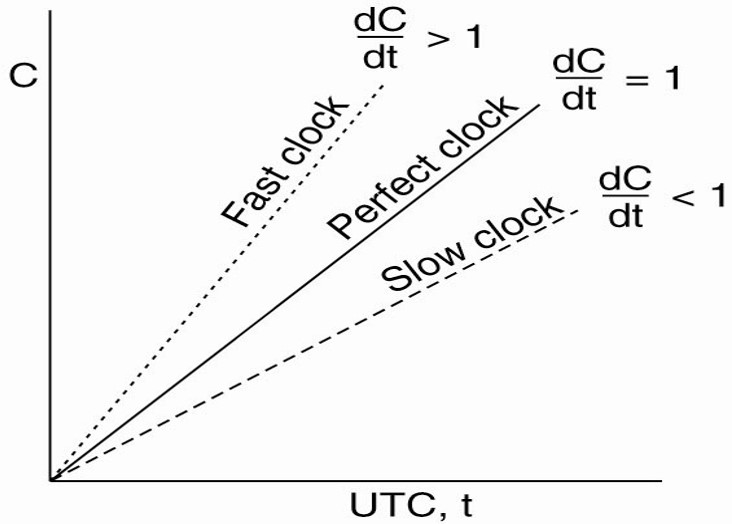
\includegraphics{Media/ClockSkew.jpg}
    Internal clock on the y-axis, UTC on the x-axis.\\
    $\frac{dC}{dt}$ = the internal clock divided by the external clock.
    \subsection*{Clock synchronization algorithms}
    
    \chapter{Christian's algorithm}
    \begin{figure}[H]
    	\centering
        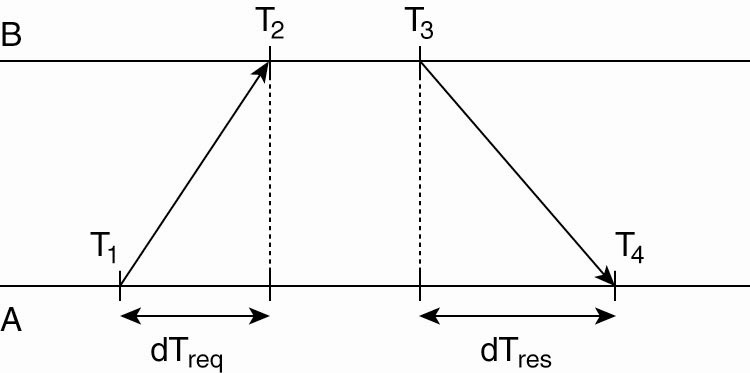
\includegraphics{Media/ChristiansAlgo.jpg}
    \end{figure}
    A's offset relative to B is $\Theta t_B-t_A$
    $$\Theta = T_2 - (T_1 + dT_{req}) = T_2 - T_1 - dT_{req}$$
    $$\Theta = T_3 - (T_4-dT_{res}) = T_3-T_4+dT_{res}$$
    $$2\Theta = (T_2-T_1)+(T_3-T_4)+(dT_{res}-dT_{req})$$
    $$\approx (T_2-T_1)+(T_3-T_4)$$
    $$t_B-t_A\approx \frac{(T_2-T_1)+(T_3-T_4)}{2}$$
    Likewise we can calculate the delay (an estimate for $dt_req$ and $dT_res$) as:
    $$\delta = \frac{(T_2-T_1)+(T_4-T_3)}{2}$$
    
    Do this a number of times and pick $\Theta$ where the delay, i.e. $\delta$, is smallest.
    
    \chapter{Berkeley algorithm}
    \begin{figure}[H]
	    \centering
	    \begin{subfigure}[b]{0.3\textwidth}
	        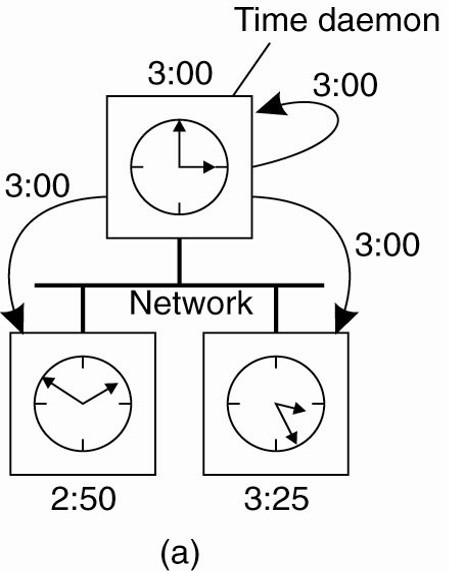
\includegraphics[width=\textwidth]{Media/Berkeley1.jpg}
	    \end{subfigure}
	    \begin{subfigure}[b]{0.3\textwidth}
	        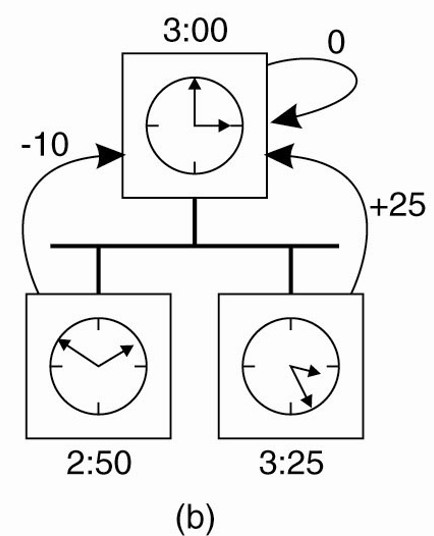
\includegraphics[width=\textwidth]{Media/Berkeley2.jpg}
	    \end{subfigure}
	    \begin{subfigure}[b]{0.3\textwidth}
	        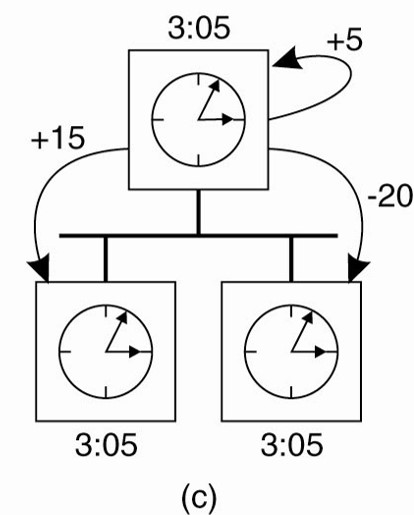
\includegraphics[width=\textwidth]{Media/Berkeley3.jpg}
	    \end{subfigure}
    \end{figure}
    
    \chapter{Logical time}
    When you just need a well-defined ordering of events and not physical time. For example an online-forum, where we want all answers to be posted after the questions and we want all answers to be in the same order on all replicas of the forum.\\
    That is, all we care about is whether event A \textit{happened before} event B.
    
    \section{The happens-before relation}
    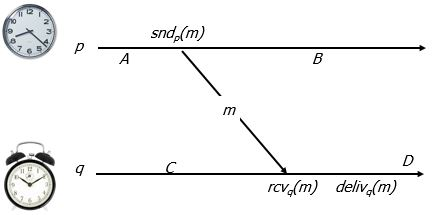
\includegraphics{Media/Time-Line.jpg}
    
    \subsection*{Local ordering}
    A happens before $snd_p(m)$ which happens before B, and C before $rcv_q(m)$ which happens before D.\\
    This is the local ordering, at each individual process, denoted:
    $$A\overset{p}{\rightarrow}snd_p(m)\overset{p}{\rightarrow}B$$
    And
    $$C\overset{q}{\rightarrow}rcv_q(m)\overset{q}{\rightarrow}D$$
    
    \subsection*{Distributed ordering}
    $snd_p(m)$ happens before $rcv_q(m)$, this is the distributed ordering of the system, denoted:
    $$snd_p(m)\overset{M}{\rightarrow}rcv_q(m)$$
    
    \subsection*{Transitive ordering}
    Since $A\rightarrow snd_p(m)$ and $snd_p\rightarrow rcv_q(m)$ we get that $A\rightarrow rcv_q(m)$ and therefore $A\rightarrow D$.
    
    \subsection*{Concurrent ordering}
    $B$ and $D$ are \textit{concurrent}, even though it looks like B happens before D, there is know way of knowing since no information have flowed between the two processes.
    
    \section{Logical clocks}
    Each process holds a local counter $C_p$ (integer) and everytime an event that matters to $p$ happens at a process $p$, the process increments $C_p$.\\
    When $p$ sends $m$ it sets:
    $$C_m=C_p$$
    When $q$ receives $m$ set:
    $$C_q=max(C_q,C_m)+1$$
    
    From previous image:
    $$C(A)=1, C(snd_p(m))=2,C(m)=2,C(B)=3$$
    $$C(C)=1,C(rcv_q(m))=max(1,2)+1=3,C(deliver_q(m))=4,C(D)=5$$
    \subsection*{Comparison with Happens-Before}
    If $A\overset{p}{\rightarrow} B$ then $C(A)<C(B)$\\
    If $A\overset{M}{\rightarrow}B$ then $C(B)=C(A)+1$\\
    If not $A\overset{p}{\rightarrow}B$ or $A\overset{M}{\rightarrow}B$, and there exist C such that $A\rightarrow C\rightarrow B;$ induction says $C(A)<C(C)$ and $C(C)<C(B)$, so $C(A)<C(B)$.\\
    \\
    \textbf{But,} $C(A)<C(B)\notimplies A\rightarrow B$.\\
    \textbf{Because,} processes that don't communicate still assign timestamps and hence events will "seem" to have an order.\\
    For example:
    \begin{figure}[H]
    \centering
    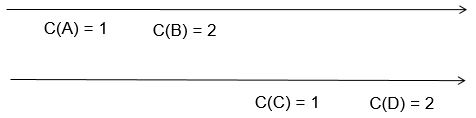
\includegraphics{Media/clockvshappensbefore.jpg}
    \end{figure}
    So $C(C)<C(B)$ but we don't have $C\rightarrow B$.
    
    
\end{document}